\documentclass[class=book, crop=false, oneside, 12pt]{standalone}
\usepackage{standalone}
\usepackage{../../style}
\graphicspath{{./assets/images/}}

% arara: pdflatex: { synctex: yes, shell: yes }
% arara: latexmk: { clean: partial }
\begin{document}
\chapter{Analisi sintattica: bottom-up parsing}
Iniziamo la trattazione del parsing di tipo \emph{bottom-up}: come suggerisce il nome stesso, consiste nel ricostruire le derivazioni di una parola in ordine inverso, partendo dall'ultima produzione e arrivando infine allo start symbol; a livello visivo, possiamo pensare che la nostra intenzione è di partire dalle foglie di un albero di derivazione e risalirlo fino alla radice.

\section{Classi di grammatiche}
Possiamo subito anticipare che anche in questo approccio possiamo identificare diversi classi di grammatiche, ciascuna delle quali ci permetterà di utilizzare, di volta in volta, diverse tecniche di parsing; in ogni caso, ciascuna di queste classi condivide le seguenti caratterstiche:
\begin{itemize}
    \item per qualsiasi grammatica \(\G\) considerata, andremo sempre a espandere il suo insieme \(\P\) in \(\P'\) aggiungendo la produzione \(S \to S'\), dove \(S'\) è un non-terminale \emph{fresh};
    \item utilizzano i medesimi algoritmi \emph{shift} e \emph{reduce} (ne parleremo più avanti);
    \item hanno sempre un automa a stati finito, detto \emph{automa caratteristico}, il cui ruolo è di supervisionare il funzionamento dell'algoritmo di parsing.
\end{itemize}
Dipendentemente dalla classe di grammatica considerata, avremo automi caratteristici che rappresentano le informazioni in maniera più o meno dettagliata. Maggiore è il livello di dettaglio dell'informazione, più diventa grande e complesso l'automa caratteristico, ma anche più potente diventail nostro parsing, inteso come numero di diverse grammatiche che può analizzare. Impariamo a conoscere qual è il significato delle abbreviazioni che costituiscono quei nomi un po' criptici delle classi di grammatiche:
\begin{labeling}{LA}
    \item[L] left: leggiamo l'input da sinistra;
    \item[R] ricostruiamo una derivazione rightmost;
    \item[1] andiamo a considerare un simbolo alla volta;
    \item[LA] sta per look ahead;
    \item[S] sta per simple;  
\end{labeling}
Noi diciamo che una grammatica \(\G\) appartiene a una certa classe, ad esempio LR(1), se \(\G\) può essere costruita con la tecnica sottesa al bottom-up parsing di tipo LR(1), vale a dire quando saremo capaci di definire una tabella deterministica che ne rispetti i vincoli.

Tra quelli presentati, il meccanismo più potente è LR(1), complementare di LL(1); per questo motivo noi cercheremo sempre di costruire una tabella di parsing deterministico che rientri nei vincoli di LR(1). Se questo non sarà possibile andremo a scalare in complessità con LALR e SRL.

\section{Un primo esempio di applicazione}
\subsection{Mosse di shift e reduce}
Andiamo a introdurre l'algoritmo che utilizzeremo per verificare se una certa parola appartenga o meno al linguaggio denotato da una certa grammatica, rappresentata dal suo automa caratteristico; questo è detto algoritmo di shift/reduce, dalle due mosse che utilizziamo:
\begin{enumerate}
    \item la mossa di \emph{shift} è quella che compiamo quando passiamoo da un nodo (stato) all'altro, inserendo nella pila delle derivazioni parziali il terminale che marca l'arco attraversato e nella pila degli stati il nodo di destinazione;
    \item la mossa di \emph{reduce} è quella che eseguiamo quando raggiungiamo un nodo marchiato da una formula di riduzione (capiremo nell'esempio quale forma hanno) e che ci porta a eliminare dei terminali dalla pila delle derivazioni parziali e degli stati dalla pila degli stati, coerentemente alla struttura dell'automa caratteristico.
\end{enumerate}
Consideriamo come esempio una delle prime grammatiche che abbiamo visto, quella che genera due occorrenza bilanciate:
\begin{equation*}
    \label{balanced}
    \G: S \to aSb \mid ab
\end{equation*}
\subsection{Esempio di automa}
L'automa caratterisco di tipo LR(1) per questa grammatica è il seguente:
\begin{figure}[H]
    \centering
    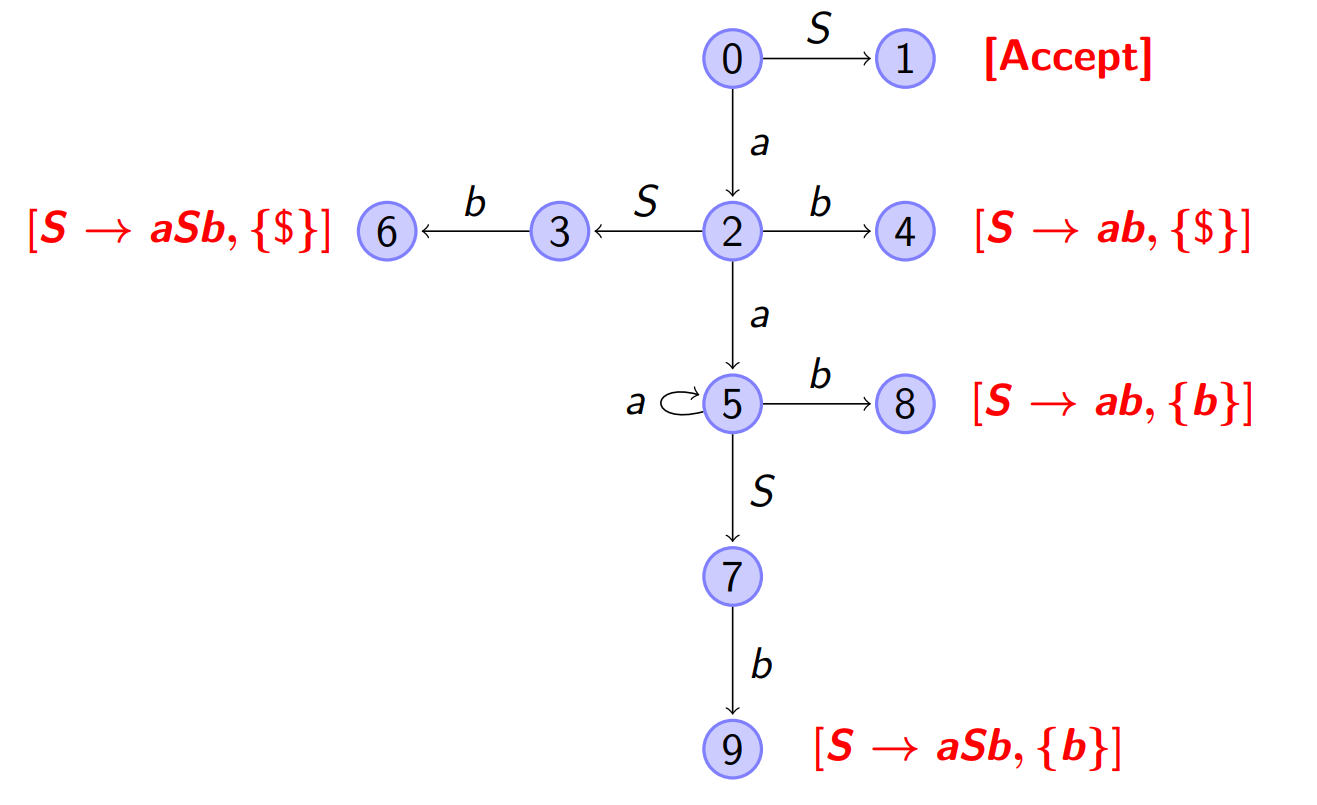
\includegraphics[width=\textwidth,keepaspectratio]{balanced-char_aut-lr1.png}
    \caption{Automa caratteristico LR(1) per Eq. \ref{balanced}}
    \label{balanced-char_aut-lr1}
\end{figure}
Lo utilizzeremo come guida per determinare, di volta in volta, quali mosse di shift e reduce applicare per verificare se una certa parola appartiene o no al linguaggio generato da \(\G\). 

\subsection{Procedura}
Consideriamo ad esempio la parola \(w = aaabbb\). Come prima cosa le applichiamo il carattere terminatore di stringa \(aaabbb\$\), e successivamente dobbiamo parlare delle strutture che utilizzeremo nella procedura, che saranno due pile:
\begin{itemize}
    \item nella prima inseriamo gli stati verso cui ci muoviamo;
    \item nella seconda conserviamo la derivazione parziale a cui siamo arrivati sinora.
\end{itemize}
Si tenga presente che in realtà potremmo farci bastare anche una sola pila, ma andrebbe a complicare sensibilmente la gestione della procedura.
\begin{itemize}
    \item Partiamo dallo stato \(0\) e inseriamolo nella pila degli stati;
    \item il primo simbolo che leggo in \(w\) è \(a\), vedo che l'automa presenta una \(a\)-transizione verso lo stato \(2\), per cui la eseguo, inserisco lo stato \(2\) nella pila, cancello il simbolo \(a\) appena "consumato" e passo al prossimo simbolo;
    \item il prossimo simbolo è ancora \(a\); di nuovo, eseguo la \(a\)-transizione verso lo stato \(5\), lo inserisco nella pila degli stati, elimino il simbolo consumato e vado avanti;
    \item abbiamo una terza occorrenza di \(a\) e abbiamo una \(a\)-transizione in forma di self loop in \(5\), che andiamo ad eseguire, reinserendo \(5\) nella pila degli stati e cancellando la nostra terza \(a\);
    \item troviamo quindi una \(b\), per cui ci spostiamo allo stato \(8\), il quale ha un'etichetta rossa, che riporta la formula \(S \to ab, \{b\}\); questo sta a indicare che, se abbiamo appena letto due simoli \(ab\), possiamo ritornare indietro di due passi, eliminando i due precedenti stati dalla pila e spostarmi direttamento dal primo \(5\) a \(7\), dal momento che i due stati sono collegati da una \(S\)-transizione:
    \begin{align*}
        \textrm{pila degli stati prima:} &\quad 02558 \\
        \textrm{pila degli stati dopo:} &\quad 0257 
    \end{align*}
    inoltre dobbiamo anche rimuovere gli ultimi due simboli \(ab\) dalla pila della derivazione e sostituirli con \(S\):
    \begin{align*}
        \textrm{pila di derivazione prima:} &\quad \#aaab \\
        \textrm{pila di derivazione dopo:} &\quad \#aaS 
    \end{align*}
    \item leggiamo un'altra \(b\) e avanziamo allo stato \(9\), e anche qui operiamo un passo di riduzione (reduce), nello specifico abbiamo che \(R: S \to aSb, \{b\}\); questo ci dice che dobbiamo tornare indietro di tre passi, eliminando i tre elementi precedenti sia nella pila degli stati e muovendoci verso \(3\), sia nella pila delle derivazioni; si osservi attentamente il cambiamento delle pile per capire cosa succede:
    \begin{align*}
        \textrm{pila degli stati prima:} &\quad 02579 & \textrm{pila di derivazione prima:} &\quad \#aaSb \\
        \textrm{pila degli stati dopo:} &\quad 023 & \textrm{pila di derivazione dopo:} &\quad \#aS
    \end{align*}
    \item proseguo quindi con la lettura e incontro una terza \(b\), mi muovo verso \(6\) e incontro una terza riduzione \(R: S \to aSb, \{\$\}\); di nuovo, torno indietro di tre stati e contestualmente sostituisco gli elementi nelle pile: 
    \begin{align*}
        \textrm{pila degli stati prima:} &\quad 0236 & \textrm{pila di derivazione prima:} &\quad \#aSb \\
        \textrm{pila degli stati dopo:} &\quad 0 & \textrm{pila di derivazione dopo:} &\quad \#S
    \end{align*}
    \item abbiamo terminato: ci troviamo nello stato \(0\) e troviamo solamente il nostro start symbol \(S\), che ci permette  muoverci verso lo stato \(1\), e l'endmaker \$; la presenza della keyword \(ACCEPT\) nello stato in cui abbiamo terminato ci indica che la parola è stata riconosciut dall'automa.
\end{itemize}

\subsection{Riassumendo}
Questo è un esempio del procedimento dell'algoritmo di shift/reduce; vediamo quali regole generali possiamo dedurne:
\begin{itemize}
    \item partendo dallo stato iniziale, inizio a leggere la parola data attraversando gli archi marchiati dalle \(symbol\)-transizioni che incontriamo di volta in volta;
    \item quando arrivo in un nodo in cui si dovrà effettuare un passo di riduzione, questo sarà marcato da un'etichetta che avrà la forma \(A \to B, \{l\}\); quello che dovrò fare a questo punto sarà scorrere all'indietro la pila delle derivazioni parziali e, se riesco a trovare un'occorrenza di quello stesso \(l\), (da capire e chiarire bene)
\end{itemize}
Gli automi caratteristici sono una rappresentazione utile, ma si tenga presente che la stessa funzione può essere ottemperata anche da una tabella.

\section{Costruzione dell'automa}
Dopo aver visto questo esempio, non possiamo fare a meno di domandarci com'è possibile per noi calcolare questo automa caratteristico e la relativa tabella di parsing.

\subsection{Stati}
Andiamo per prima cosa a vedere gli stati. Gli stati sono degli insiemi di items, dove gli items sono oggetti di diverso tipo e così definiti:
\begin{labeling}{LR(1)-items}
    \item[LR(0)-items] \(A \to \alpha \cdot \beta\)
    \item[LR(1)-items] [\(A \to \alpha \cdot \beta, L\)], dove \(L \subseteq T \cup \{\$\}\)\footnote{Ricordiamo che \(T\) è l'insieme dei terminali della grammatica considerata.}
\end{labeling}
Da qui capiamo finalmente cosa intendevamo quando prima abbiamo detto che gli LR(1)-items sono più ricchi dei loro equivaleenti LR(0), e ci permettono quindi di riconoscere più grammatiche. Coerentemente alla definzione sopra riportata, avremo che gli automi caratteristici LR(0) sono quelli i cui stati sono LR(0)-items, e analogamente per gli automi carattersitici LR(1).

Andiamo a fare subito un esempio per aiutarci a capire di cosa stiamo parlando. Consideriamo un LR(0)-item \(S' \to \cdot S\): il significato intuitivo è che, se siamo all'inizio della procedura di parsing, siamo in una posizione in cui vogliamo conoscere quali sono le parole derivabili a partire da \(S\), per cui è logico pensare che il nostro item \(S' \to \cdot S\) debba stare nello stato iniziale dell'automa, che chiamiamo \(P_0\).

Ma non sarà l'unico item a risiedere in \(P_0\). Per aiutarci, riprendiamo la nostra fidata grammatica in Eq. \ref{balanced}: in questo caso, analizzare la parola vuol dire aspettarsi qualcosa che derivi da \(aSb\) oppure \(ab\), per cui gli LR(0)-items di \(S\) saranno:
\begin{itemize}
    \item \(S \to \cdot aSb\);
    \item \(S \to \cdot ab\).
\end{itemize}
E verranno inseriti in \(P_0\).

\subsection{Chiusura di un insieme di LR(0)-items}
Andiamo ora a vedere il concetto di chiusura di un insieme di LR(0)-items:

\begin{definition}
    Sia \(P\) un insieme di LR(0)-items; allora, \(closure_0(P)\) è il più piccolo insieme che soddisfa la seguente equazione:
    \begin{equation}
        closure_0(P) = P \cup \{B \to \cdot \gamma \; \textrm{tale che} \; A \to \alpha \cdot B \beta \in closure_0(P) \; \textrm{e} \; B \to \gamma \in P'\}
    \end{equation}
\end{definition}

La chiusura consiste sostanzialmente in tutti quegli items che hanno un punto davanti ad un non terminale; poi, ricorsivamente, si vanno ad aggiungere tutte le chiusure dei terminali con un punto davanti.

\end{document}